\chapter {Execução dos Testes e Análise dos Resultados}

Nesse capítulo vamos descrever o ambiente onde os testes foram realizados, as métricas que foram escolhidas para medir a performance e os resultados obtidos.

\section{Ambiente de testes}

Os testes foram realizados em uma máquina física com as seguintes configurações:

\begin{itemize}
\item Sistema Operacional: Debian GNU/Linux 6.0
\item Processador: Intel Pentium Quad Core
\item Quantidade de Memória RAM: 4 GB
\item MongoDB: Versão 2.4.0 padrão
\item PostgreSQL: Versão 8.4.16 padrão
\item Driver Python MongoDB: pymongo
\item Driver Python PostgreSQL: psycopg
\end{itemize}

\section{Massa de Dados}

Conforme Molyneaux diz ~\cite{theartoftestperf}, a importância de prover a quantidade de dados de qualidade para um teste não pode ser exagerada. Segundo ele, a quantidade e a qualidade dos dados podem definir o sucesso ou insucesso dos testes. Para o nosso projeto foi desenvolvido um script em python para a geração da massa de dados. Os dados podem tanto ser inseridos diretamente na base de dados quanto em arquivos CSV, os quais serão utilizados durante os testes. Os arquivos (documentos para simular a pasta funcional) utilizados nos testes possuem tamanho médio de 400 KB. A não ser pela diferença das chaves primárias geradas nos dois bancos, os dados inseridos no MongoDB e no PostgreSQL são iguais. A quantidade de dados gerados também pode ser configurada pelo seguinte:

\begin{enumerate}
	\item Quantidade de Unidades Pagadoras (Orgãos);
	\item Quantidade de empregados por orgão;
	\item Quantidade de dependentes por empregado;
	\item Quantidade de documentos por empregado;
	\item Quantidade de documentos por dependente;
\end{enumerate}

A quantidade de dados utilizados pode ser vista na tabela \ref{tab:massadadosutil}

\begin{table}
	\caption{Massa de Dados Utilizada}
	\begin{center}
	\begin{tabularx}{\textwidth}{ | c | X | }
	\hline
		\multicolumn{2}{|c|}{\textbf{Massa de Dados}} \\
	\hline
		Quantidade de Unidades Pagadoras (Órgãos) &  10\\
	\hline
		Quantidade de empregados por orgão & 100\\
	\hline 
		Quantidade de dependentes por empregado & 2 \\
	\hline
		Quantidade de documentos por empregado & 5\\
	\hline
		Quantidade de documentos por dependente & 2\\
	\hline
		Quantidade de dependentes excluídos & 250\\
	\hline
		Quantidade de empregados desligados & 250\\
	\hline
	\end {tabularx}
	\end{center}
	\label{tab:massadadosutil}
\end{table}

\section{Métricas}

Quando se quer balancear o custo e a performance, todos os envolvidos na produção do software se preocupam com a execução de testes de performance. A avaliação de performance é necessária em todas as etapas do ciclo de vida de software e é requerida sempre que o arquiteto precisa comparar alternativas~\cite{rajjain}. Em um teste de performance a escolha das métricas é de grande importância. Segundo Raj Jain ~\cite{rajjain}, escolher as métricas erradas é um dos erros mais comuns. Nesse trabalho a performance será avaliada pelo tempo médio de resposta.

\section{Resultados}

Como podemos ver nos gráficos apresentados a seguir, a performance dos dois bancos foram bastante próximas. Após executar os testes, foram salvos os tempos de todas as requisições feitas à aplicação e calculado o tempo médio de resposta, em milisecundos, para cada teste realizado.

Para os testes de consulta, exceto no teste 'Consulta Documentos do Dependente' o MongoDB sempre foi mais lento em relação ao PostgreSQL.

Na inserção de orgãos os tempos foram muito próximos e, como a quantidade de registros inseridos foram poucos, podemos dizer que a performance dos dois bancos foram iguais.

Ao inserir os dados dos empregados e dos dependentes, trabalhamos com uma quantidade de registros maior e assim podemos ver que o MongoDB foi sempre mais lento em relação ao PostgreSQL. Essa diferença de performance foi aumentando à medida em que a quantidade de usuários simultâneos foi incrementada.

No teste 'Consulta Usuários Ativos' é feito um cálculo interno e também foi utilizado agrupador nas consultas realizadas nos dois bancos. Mais uma vez o PostgreSQL foi mais rápido ao responder as requisições.

Ao testarmos a inserção de documentos, tanto de empregados quanto dos seus dependentes,percebemos que o tempo de resposta aumentou muito em relação aos outros testes. Isso se deve ao fato de que foram adicionalmente necessárias operações de criação e leitura de arquivos e diretórios. Esses testes foram realizados apenas para 10 e 100 usuários simultâneos, pois a arquitetura não nos permitiu mais. Ao inserir os documentos dos empregados podemos ver que a diferença se mostra maior ao testarmos com 100 usuários simultâneos, quando o PostgreSQL é aproximadamente um segundo mais rápido que o MongoDB. Já na inserção dos documentos dos dependentes, a performance dos dois bancos são bem parecidadas, com uma pequena vantagem para o MongoDB.

Ao testarmos a atualização de registros no teste 'Desliga Empregado' e a exclusão de registros no teste 'Remove Dependente', mesmo com operação de \textit{join} nesse, também foi verificado que o PostgreSQL é mais rápido ao responder às requisições.

Ao final dos testes pode-se verificar que nenhum banco de dados foi consideravelmente mais veloz que o outro e que, para praticamente todos os testes realizados, o PostgreSQL se mostrou mais rápido. Dessa maneira, para o cenário de manutenção dos dados do AFD, com a arquitetura, massa de dados e modelagem utilizadas, não é vantajoso utilizar o MongoDB para a persistência dos dados, visto que, mesmo com todos os recursos de segurança e controle de transações oferecidos pelo PostgreSQL, ele ainda continua sendo mais performático.


\begin{figure}[!htbp]
	\begin{center}
		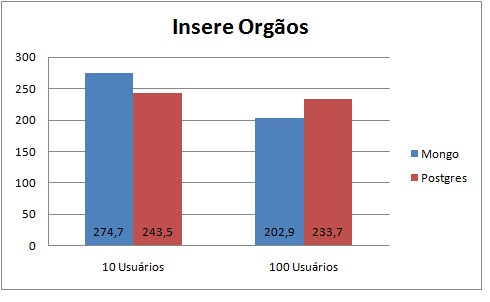
\includegraphics[width=0.8\textwidth]{resultados/insere_orgaos}
	\end{center}
	\caption{Resultados - Insere Órgãos}
	\label{fig:resultinsereorgaos}
\end{figure}

\begin{figure}[!htbp]
	\begin{center}
		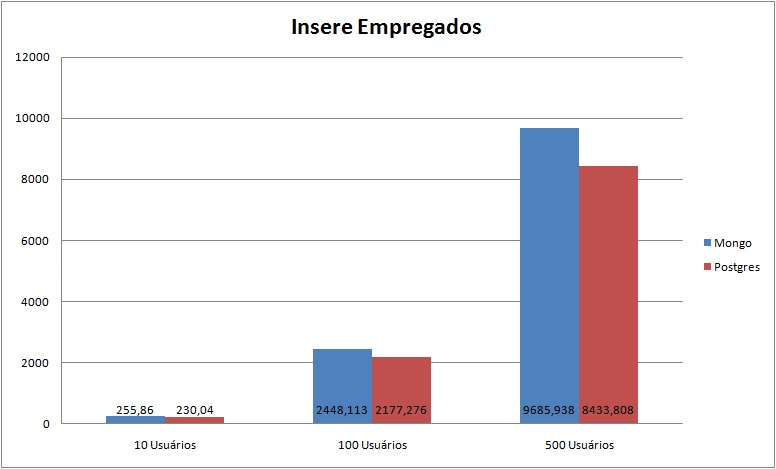
\includegraphics[width=0.8\textwidth]{resultados/insere_empregados}
	\end{center}
	\caption{Resultados - Insere Empregados}
	\label{fig:resultinsereempregados}
\end{figure}

\begin{figure}[!htbp]
	\begin{center}
		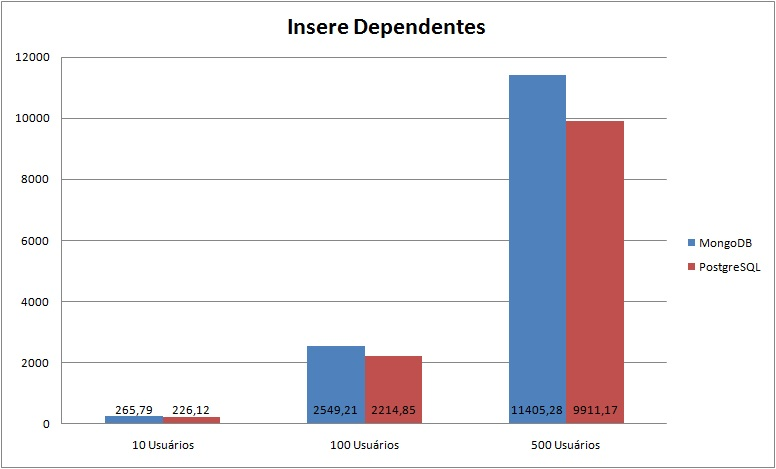
\includegraphics[width=0.8\textwidth]{resultados/insere_dependentes}
	\end{center}
	\caption{Resultados - Insere Dependentes}
	\label{fig:resultinseredependentes}
\end{figure}

\begin{figure}[!htbp]
	\begin{center}
		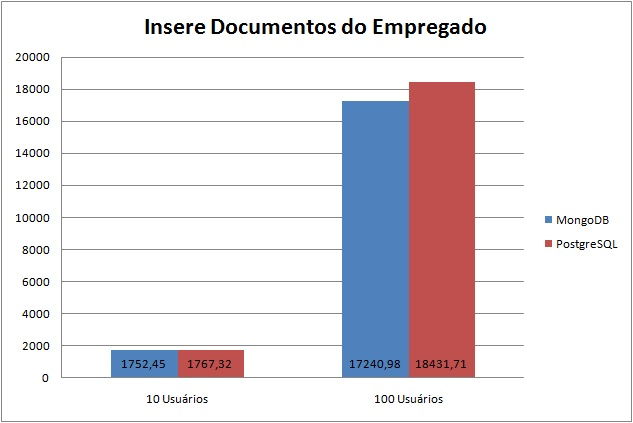
\includegraphics[width=0.8\textwidth]{resultados/insere_doc_empregado}
	\end{center}
	\caption{Resultados - Insere Documento do Empregado}
	\label{fig:resultinseredocempregado}
\end{figure}


\begin{figure}[!htbp]
	\begin{center}
		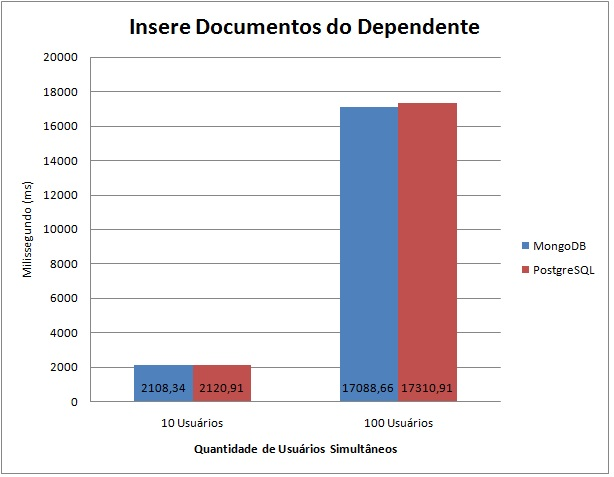
\includegraphics[width=0.8\textwidth]{resultados/insere_doc_dependentes}
	\end{center}
	\caption{Resultados - Insere Documento do Dependente}
	\label{fig:resultinseredocdependente}
\end{figure}

\begin{figure}[!htbp]
	\begin{center}
		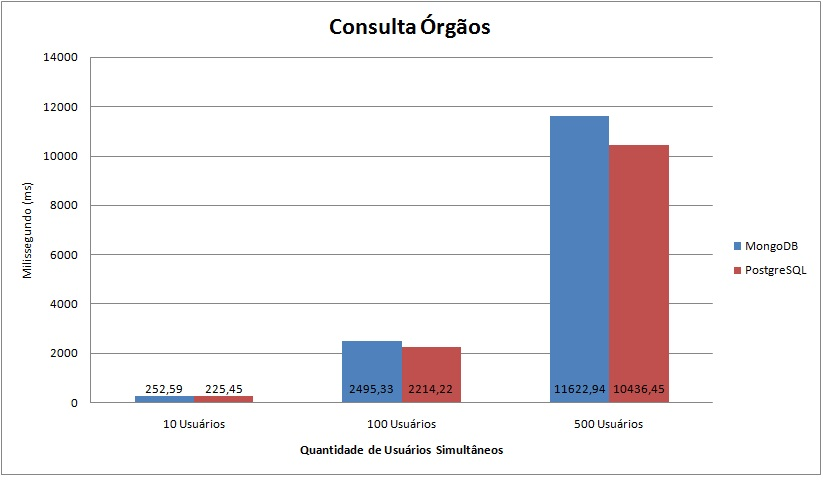
\includegraphics[width=0.8\textwidth]{resultados/consulta_orgaos}
	\end{center}
	\caption{Resultados - Lista Órgãos}
	\label{fig:resultlistaorgaos}
\end{figure}

\begin{figure}[!htbp]
	\begin{center}
		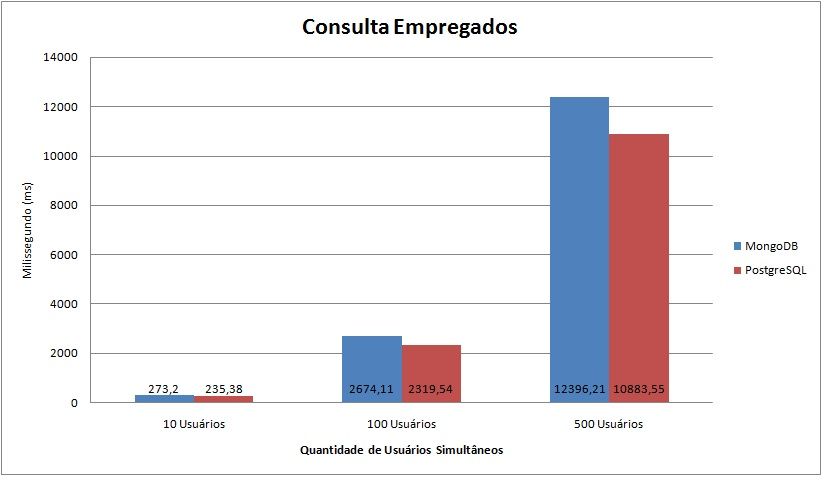
\includegraphics[width=0.8\textwidth]{resultados/consulta_empregados}
	\end{center}
	\caption{Resultados - Lista Empregados}
	\label{fig:resultlistaempregados}
\end{figure}

\begin{figure}[!htbp]
	\begin{center}
		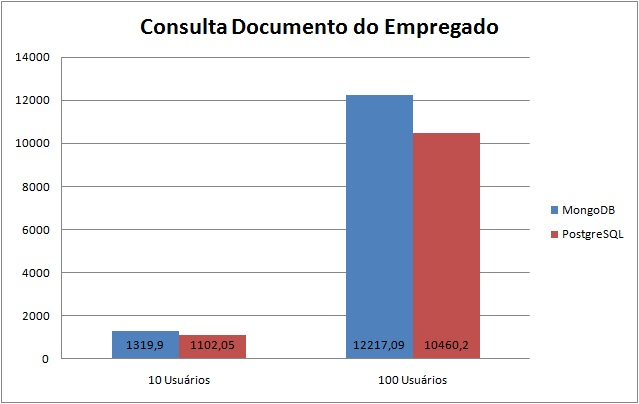
\includegraphics[width=0.8\textwidth]{resultados/consulta_doc_empregado}
	\end{center}
	\caption{Resultados - Lista Documentos do Empregado}
	\label{fig:resultlistadocempregado}
\end{figure}

\begin{figure}[!htbp]
	\begin{center}
		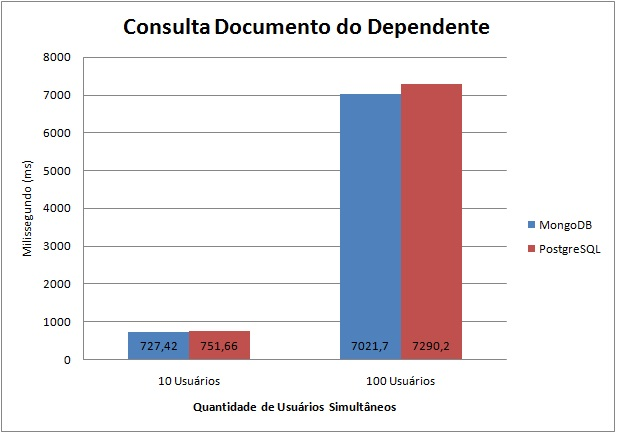
\includegraphics[width=0.8\textwidth]{resultados/consulta_doc_dependente}
	\end{center}
	\caption{Resultados - Lista Documentos do Dependente}
	\label{fig:resultlistadocdependente}
\end{figure}

\begin{figure}[!htbp]
	\begin{center}
		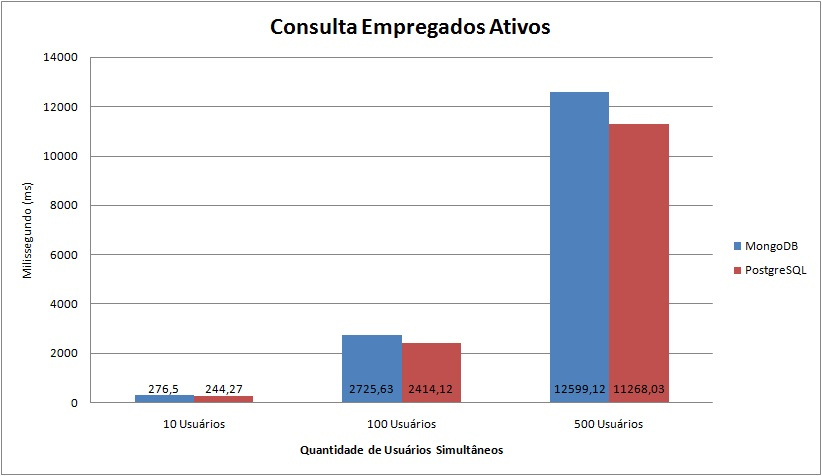
\includegraphics[width=0.8\textwidth]{resultados/consulta_estatistica}
	\end{center}
	\caption{Resultados - Consulta Empregados Ativos}
	\label{fig:resultlistaempregadosativos}
\end{figure}

\begin{figure}[!htbp]
	\begin{center}
		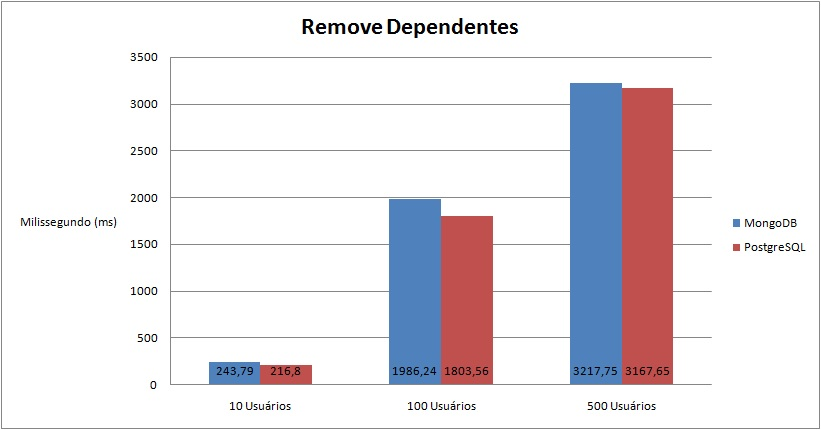
\includegraphics[width=0.8\textwidth]{resultados/remove_dependentes}
	\end{center}
	\caption{Resultados - Remove Dependentes}
	\label{fig:resultremovedependentes}
\end{figure}

\begin{figure}[!htbp]
	\begin{center}
		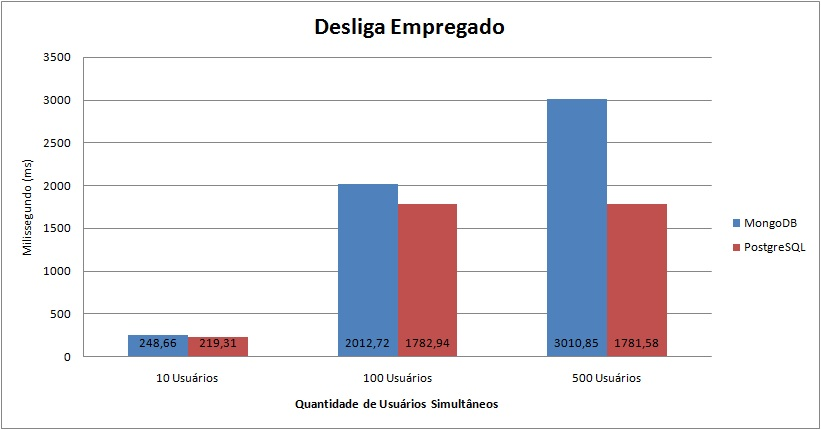
\includegraphics[width=0.8\textwidth]{resultados/desliga_empregado}
	\end{center}
	\caption{Resultados - Desliga Empregado}
	\label{fig:resultdesliga_empregado}
\end{figure}


